\documentclass{beamer}

\usepackage[english]{babel}
\usepackage[utf8]{inputenc}
\usepackage{graphicx}
\usepackage{moresize}
\usepackage{mathptmx}
\usepackage{helvet}
\usepackage{hyperref}
\usepackage[final]{pdfpages}

%\usepackage{multicol}

\usefonttheme{serif}

\definecolor{th_black}{rgb}{0.0, 0.051, 0.075}
\definecolor{th_red}{rgb}{0.8, 0.176, 0.196}
\definecolor{th_orange}{rgb}{0.827, 0.373, 0.161}
\definecolor{th_purple}{rgb}{0.616, 0.192, 0.549}
\definecolor{light_gray}{rgb}{0.741, 0.784, 0.812}
\definecolor{dark_gray}{rgb}{0.439, 0.475, 0.498}
\definecolor{title_box}{HTML}{b683ca}%{a767bf}


\setbeamerfont{title}{size=\HUGE}
\setbeamerfont{frametitle}{size=\Large, series=\bfseries}

\setbeamercolor{title}{bg=white, fg=dark_gray}
\setbeamercolor{frametitle}{bg=white, fg=dark_gray}

\setbeamercolor{section number projected}{bg=th_red}
\setbeamercolor{subsection number projected}{bg=th_purple}
\setbeamercolor{section in toc}{fg=black}
\setbeamercolor{subsection in toc}{fg=darkgray}

\setbeamercolor{header left}{bg=th_red}
\setbeamercolor{header center}{bg=th_orange}
\setbeamercolor{header right}{bg=th_purple}


\setbeamertemplate{itemize item}{\color{th_red}$\blacktriangleright$}
\setbeamertemplate{itemize subitem}{\color{th_purple}$\blacktriangleright$}
%\setbeamertemplate{itemize subsubitem}{\color{orange}$\blacktriangleright$}

\setbeamertemplate{title page}[default][left]%colsep=-4bp,rounded=true, shadow=true

\setbeamertemplate{section in toc}[ball unnumbered]
\setbeamertemplate{subsection in toc}[ball unnumbered]

\beamertemplatenavigationsymbolsempty

\setbeamertemplate{footline}{%
	\leavevmode
    \begin{beamercolorbox}[wd=0.125\paperwidth,dp=1pt]{}
    \end{beamercolorbox}%
    \begin{beamercolorbox}[wd=0.875\paperwidth]{}
    \hrule
    \vspace{0.1mm}
    \hrule
    \vspace{1mm}
    \parbox[b]{0.5\paperwidth}{\inserttitle\\[1.5mm] \insertshortauthor\\ \insertshortdate}
    \hfill
    Slide~\insertframenumber~of~\inserttotalframenumber
    \hspace{5mm}
    
\includegraphics[width=0.12\paperwidth]{sources/logo_TH-Koeln_CMYK_22pt}
    \hspace{2mm}
    \vspace{1mm}
    \end{beamercolorbox}%
}

\setbeamertemplate{headline}{%
    \leavevmode
    \begin{beamercolorbox}[wd=0.125\paperwidth,ht=1pt,dp=4pt]{}
    \end{beamercolorbox}%
    \begin{beamercolorbox}[wd=0.292\paperwidth,ht=1pt,dp=4pt]{header left}
    \end{beamercolorbox}%
    \begin{beamercolorbox}[wd=0.292\paperwidth,ht=1pt,dp=4pt]{header center}
    \end{beamercolorbox}%
    \begin{beamercolorbox}[wd=0.292\paperwidth,ht=1pt,dp=4pt]{header right}
    \end{beamercolorbox}
} 


%Information to be included in the title page:
\title{Object Hunt}
\subtitle{Final Presentation}
\author[Manuel Audran, Tim Mennicken, Robert Rose]{Manuel Audran\\ Tim Mennicken\\ Robert Rose}
\institute[TH Köln]{University of Applied Sciences Cologne}
\date[29.01.2020] % (optional)
{Wednesday the 29th of January, 2020}
%\logo{
\includegraphics[height=0.8cm]{sources/logo_TH-Koeln_CMYK_22pt}}
 
 
\begin{document}
\bgroup
\makeatletter
\setbeamertemplate{footline}
{
	\leavevmode
    \begin{beamercolorbox}[wd=0.125\paperwidth,dp=1pt]{}
    \end{beamercolorbox}%
    \begin{beamercolorbox}[wd=0.875\paperwidth,dp=0ex]{}
    \hrule
    \vspace{0.1mm}
    \hrule
    \vspace{1mm}
    \parbox[b]{0.3\paperwidth}{\inserttitle\\[1.5mm] \insertshortauthor\\ \insertshortdate}
    \hfill
    
\includegraphics[width=0.12\paperwidth]{sources/logo_TH-Koeln_CMYK_22pt}
    \hspace{2mm}
    \vspace{1mm}
    \end{beamercolorbox}%
}
\makeatother
\begin{frame}
\titlepage
\end{frame}
\egroup

\setcounter{framenumber}{0}

\begin{frame}
\frametitle{Table of Contents}
%\begin{multicols}{2}
\tableofcontents
%\end{multicols}
\end{frame} 
 
\section{Hardware}

\begin{frame}{Hardware Overview}
\begin{columns}
\column{0.5\textwidth}
\begin{itemize}
\item Ultra sonic distance sensor
\item Infrared revolution sensor
\item Smart movement sensor
\item Camera module
\end{itemize}
\vspace{5mm}
\begin{itemize}
\item<2-> DC gear motor
\item<2-> Stepper motor
\end{itemize}
 
\column{0.5\textwidth}
\includegraphics[scale=0.19]{../documentation/images/hardware_setup.png}
\end{columns}
\end{frame}

\subsection{PCB Board}

\begin{frame}{PCB Board}
\centering
\includegraphics[scale=0.098, angle=90]{../documentation/images/pcb.jpg}
\end{frame}

\subsection{Assembly}

\begin{frame}{Assembly}
\centering
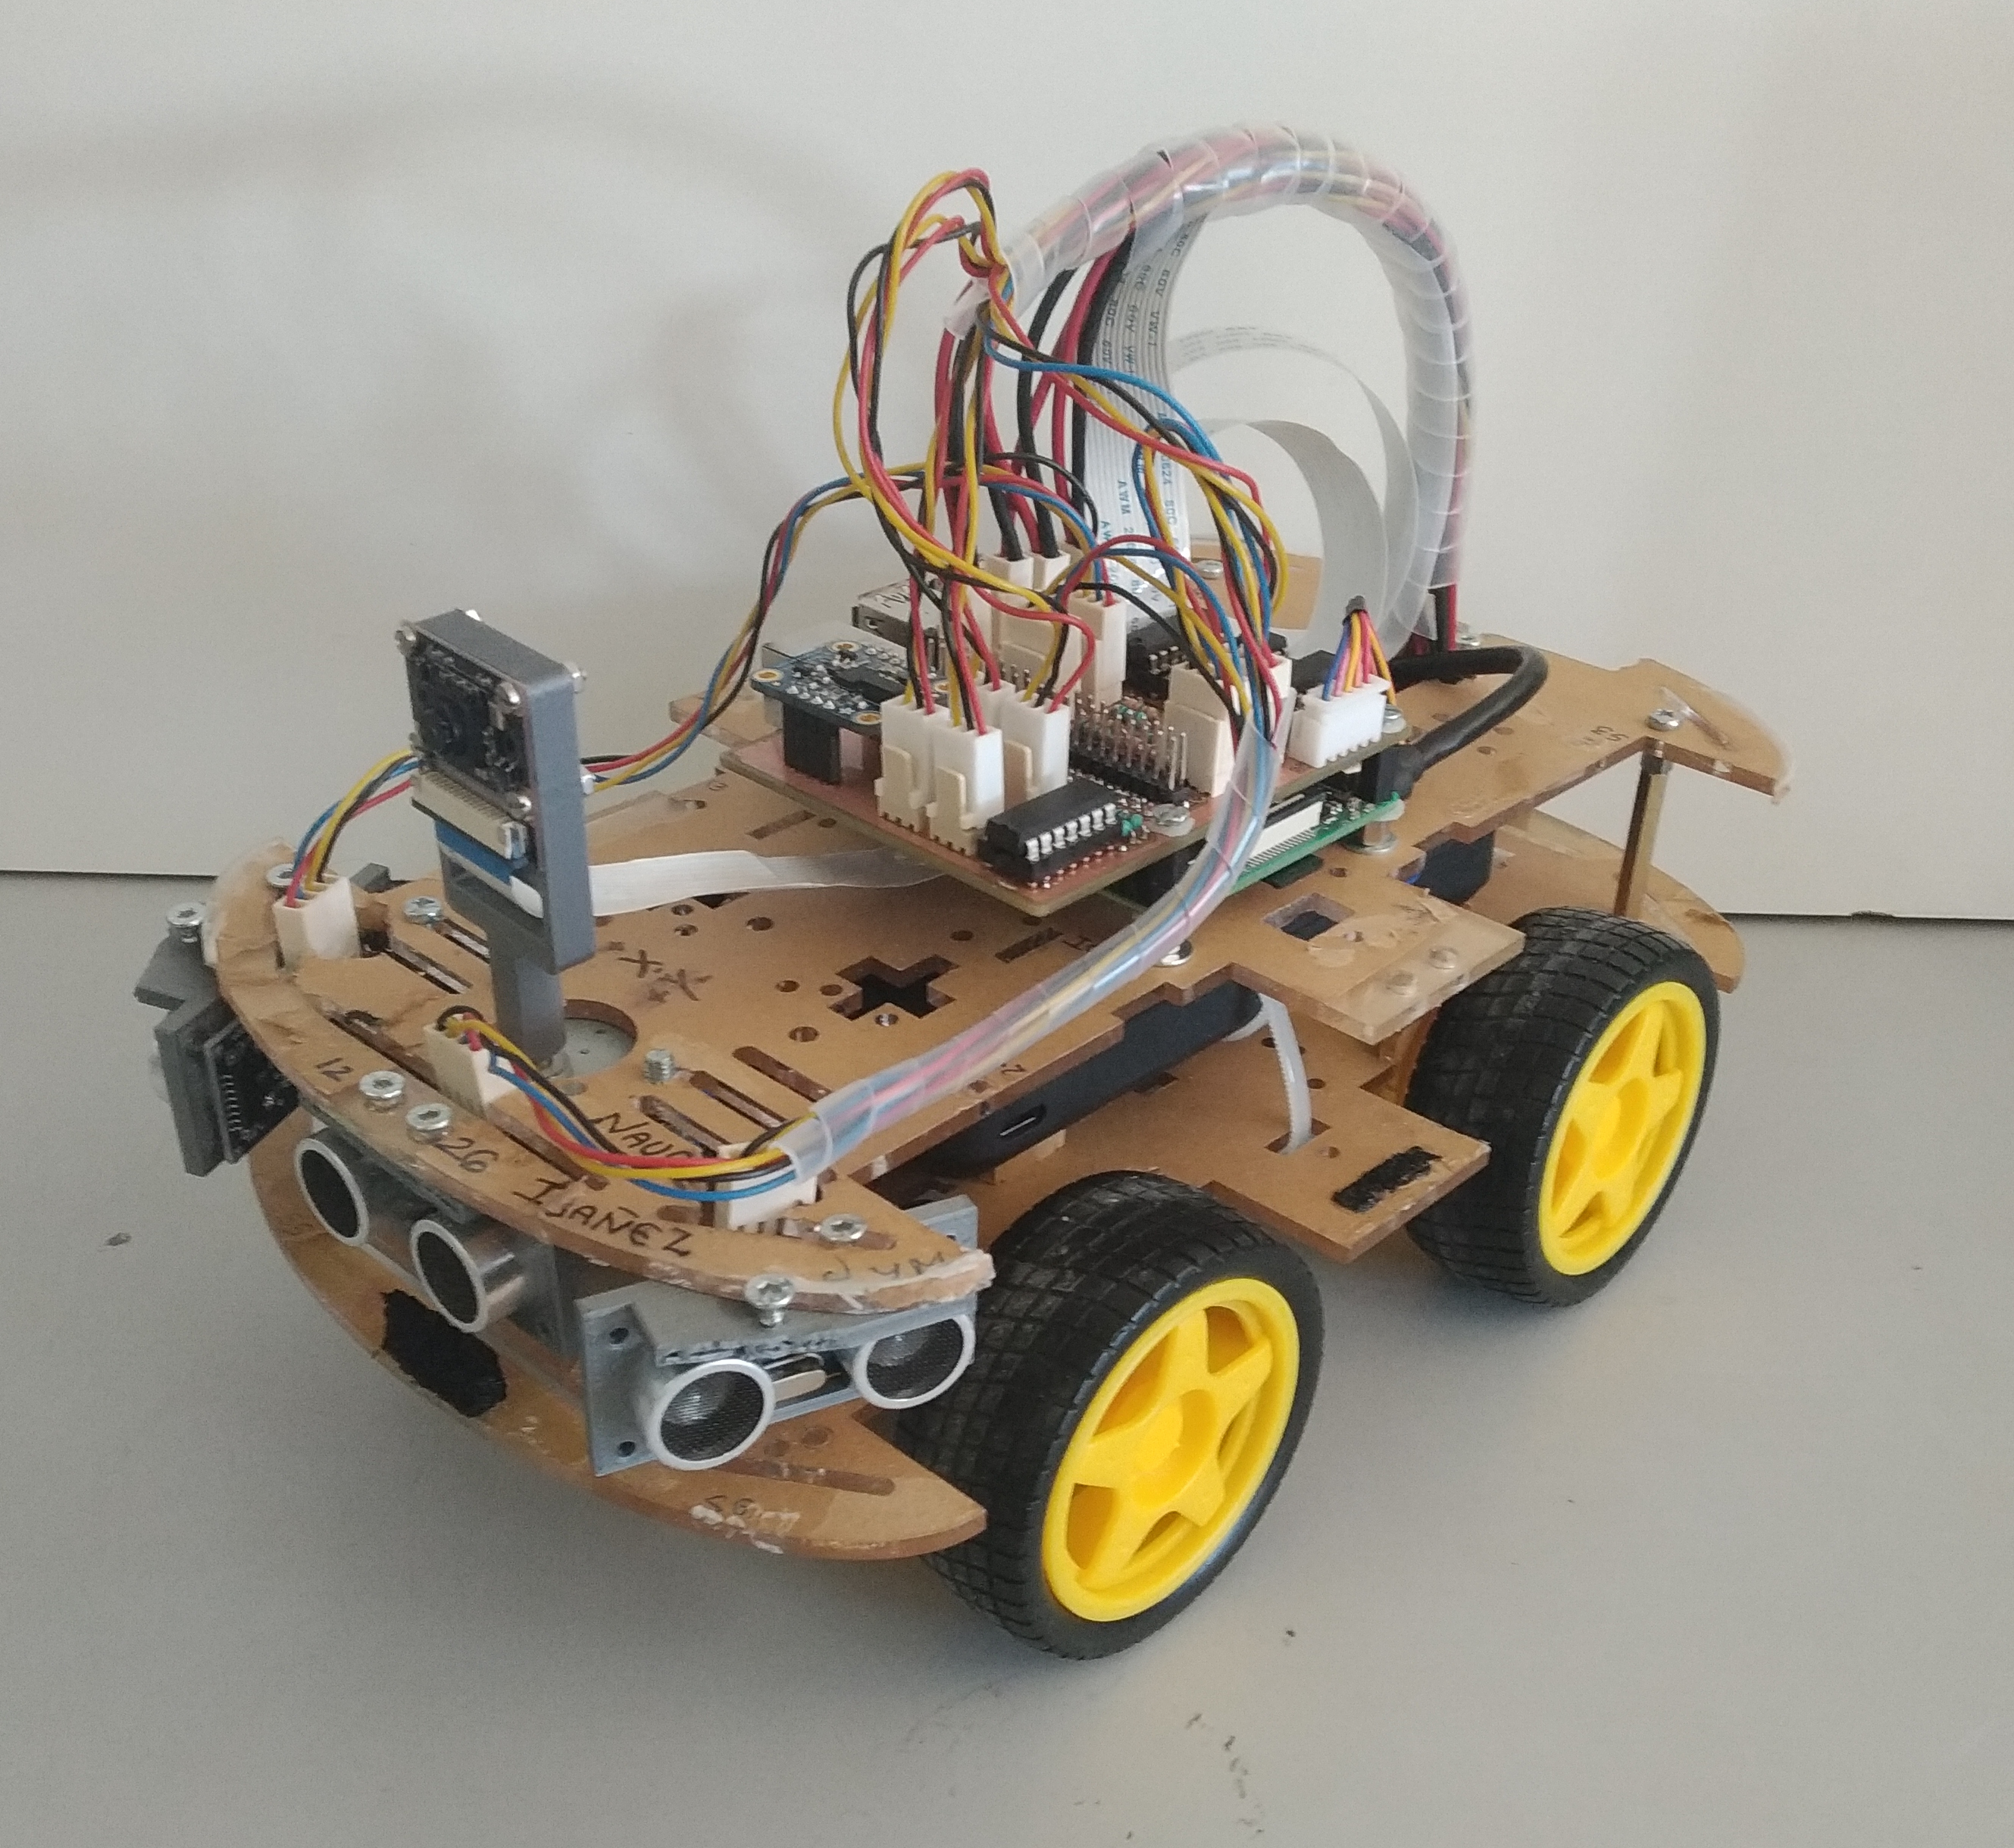
\includegraphics[scale=0.0835]{../documentation/images/car_complete.jpg}
\end{frame}

\section{Software}

\begin{frame}{Software Principles}
\begin{itemize}
\item Communication
	\begin{itemize}
	\item Via TCP/ IP
	\item Independent from other devices
	\item Beyond system border
	\end{itemize}
	\vspace{2mm}
	
\item<2-> Economical
	\begin{itemize}
	\item No unnecessary CPU consume
	\item Fast reaction times
	\item Event driven
	\end{itemize}
	\vspace{2mm}
	
\item<3-> Documentation
	\begin{itemize}
	\item Complete
	\item Easy accessible
	\end{itemize}
\end{itemize}
\end{frame}

\subsection{Inter-process communication}

\begin{frame}{Connection Overview}
\centering
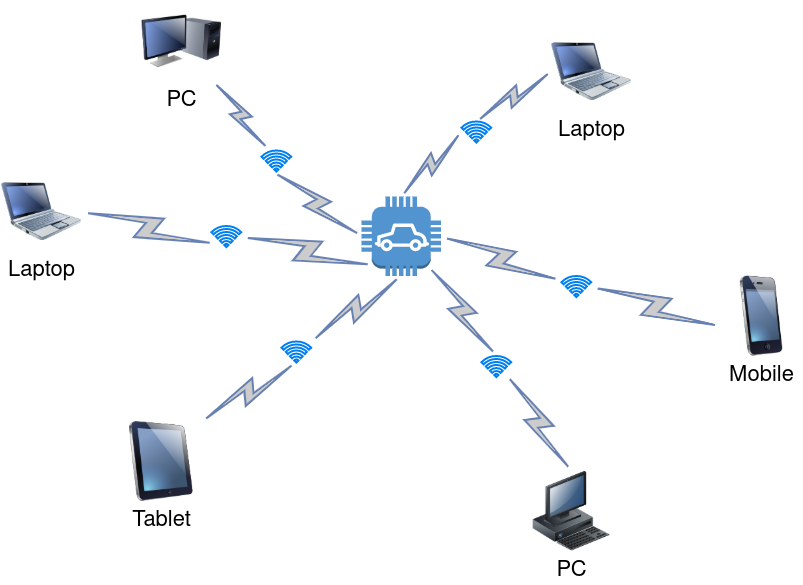
\includegraphics[scale=0.32]{../documentation/images/connection_overview.png}
\end{frame}

\begin{frame}{Connection Implementation}
\centering
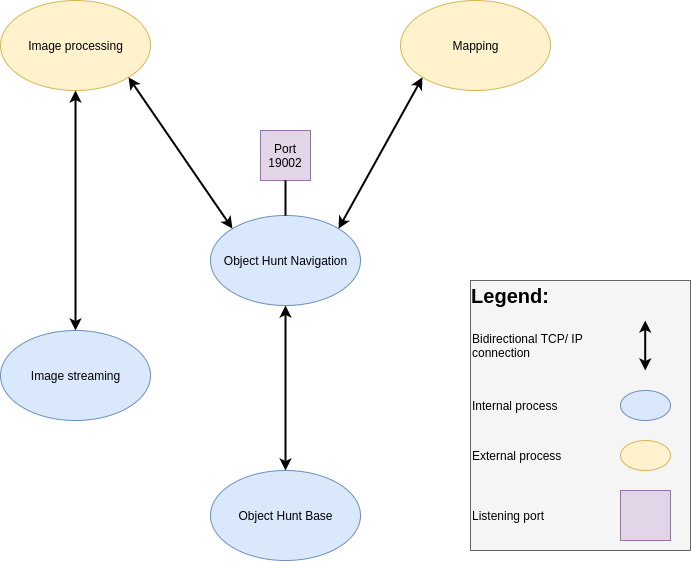
\includegraphics[scale=0.32]{../documentation/images/software_structure.png}
\end{frame}

\subsection{Internal processes}

\begin{frame}{Base Process}
\begin{itemize}
\item Exclusively accesses the hardware
\item Receives commands and requests from the navigation process
\item Continuous communication with the navigation process
\end{itemize}
\pause
\centering
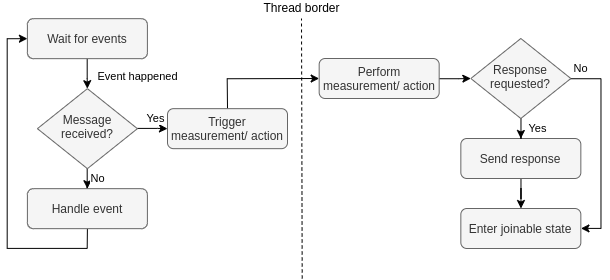
\includegraphics[scale=0.45]{../documentation/images/flowchart_base.png}
\end{frame}

\begin{frame}{Navigation Process}
\begin{itemize}
\item Requests periodically sensor readings
\item Sends navigation commands
\item Handles connections with further processes
\end{itemize}
\pause
\centering
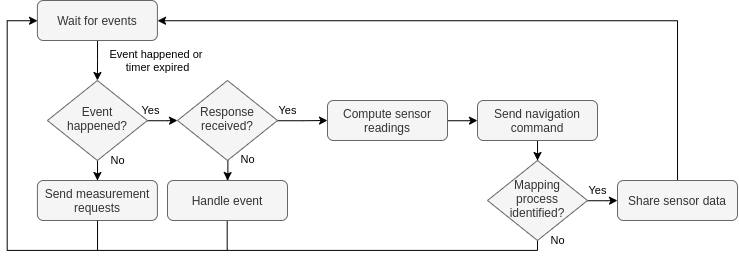
\includegraphics[scale=0.43]{../documentation/images/flowchart_navigation.png}
\end{frame}

\section{Image processing}

\subsection{Software setup}

\begin{frame}{Software Setup}
\begin{itemize}
\item Python 3.7.3
\item[]
\item OpenCV 4.1.2
\item[]
\item ImageZMQ (Python wrapper for ZMQ functionalities)
\item[]
\item MobileNet v2 SSD
\item[]
\item COCO dataset
\end{itemize}
\end{frame}

\subsection{Framework}

\begin{frame}{Framework - Open Source Computer Vision Library}
\begin{columns}
\column{0.5\textwidth}
\begin{itemize}
\item Platform independent library written in C++
\item Available as Python pip package
\item DNN module to utilize pretrained Tensorflow models
\item Offers utilization methods to present the images
\end{itemize}
\column{0.5\textwidth}
\hfill 
\includegraphics[scale=0.2]{sources/OpenCV_Logo_with_text.png}
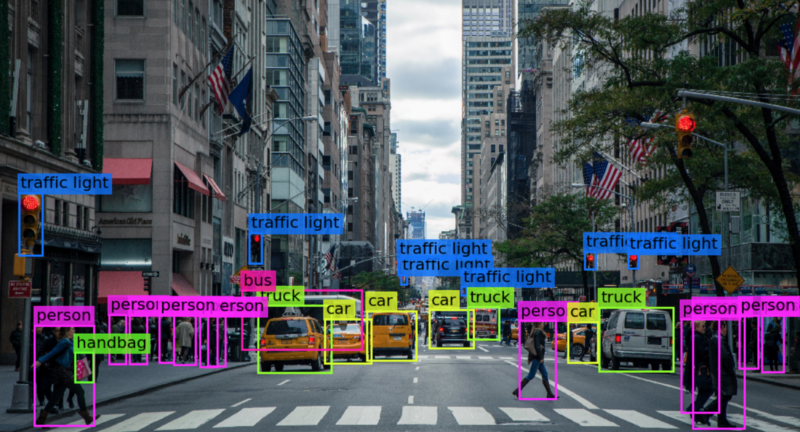
\includegraphics[scale=0.2]{sources/18.png}
\end{columns}
\end{frame}

\subsection{Streaming}

\begin{frame}{Streaming}
\begin{columns}
\column{0.55\textwidth}
\begin{itemize}
\item First analysis shows Raspberry Pi is not capable of real-time object detection
\item Solution $\Rightarrow$ stream the video and process it on the PC
\item ImageZMQ is based on ZeroMQ, made for transporting OpenCV images over network
\item Results in two processes, connected via sockets
\end{itemize}
\column{0.45\textwidth}
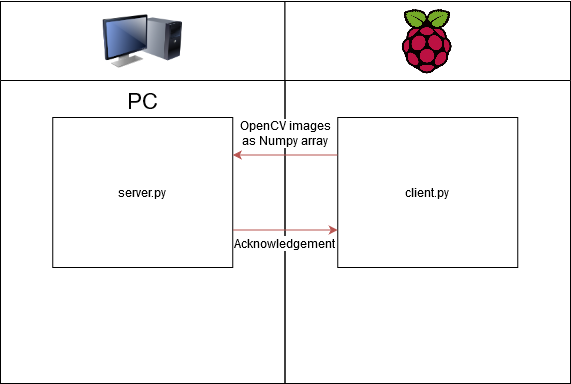
\includegraphics[scale=0.26]{sources/diagram.png}
\end{columns}
\end{frame}

\subsection{Model}

\begin{frame}{Model}
\begin{itemize}
\item[] Requirements:
\item Object detection (tennis ball as defined object)
\item Real-time processing
\item Sufficient accuracy
\end{itemize}
\vspace{1cm}
\begin{itemize}
\item[]$\Rightarrow$ MobileNet in combination with SSD offers an efficient solution for embedded systems with real-time object detection
\item[]$\Rightarrow$ COCO dataset includes 90 different classes
\end{itemize}
%$\Rightarrow$ Mobilenet in combination with SSD offers an efficient solution for embedded systems with real-time object detection
%$\Rightarrow$ COCO dataset includes 90 different classes
\end{frame}

\begin{frame}{Model - Mobilnet Architecture}
\begin{columns}
\column{0.65\textwidth}
\begin{itemize}
\item Main difference: Depthwise separable convolution
\item Splits up convolution in two parts
	\begin{itemize}
	\item 3x3 depthwise Conv
	\item 1x1 pointwise Conv
	\end{itemize}
\item Reduces the number of trainable parameters remarkably
\item Trade-off is less accuracy
\end{itemize}
\column{0.35\textwidth}
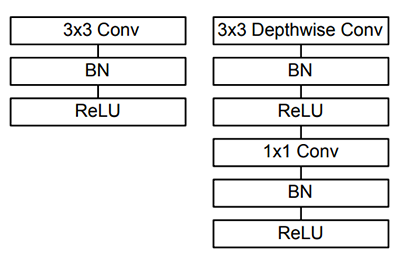
\includegraphics[scale=0.3]{sources/mobilenet_depthwise.png}
\end{columns}
\end{frame}

\begin{frame}{Model – Single Shot Detection}
\begin{columns}
\column{0.5\textwidth}
\begin{itemize}
\item Defines default boxes
\item Generates scores for each category and default box
\item Adjusts the box to match the object shape
\vspace{5mm}
\item Three commonly used object detection methods:
	\begin{itemize}
	\item Faster R-CNN
	\item YOLO
	\item SSD
	\end{itemize}
\end{itemize}
\column{0.5\textwidth}
\hfill 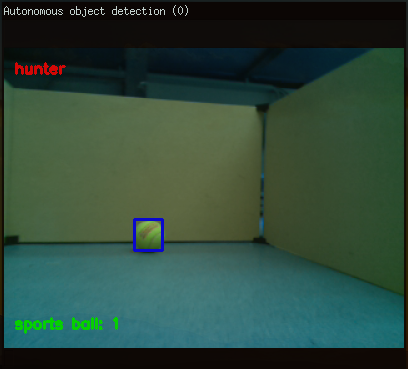
\includegraphics[scale=0.35]{sources/ss.png}
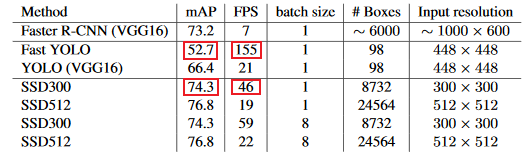
\includegraphics[scale=0.4]{sources/tempsnip.png}
\end{columns}
\end{frame}

\section{Mapping \& Routing}

\begin{frame}{Mapping \& Routing}
\centering
\begin{figure}
\begin{overprint}
	\onslide<1>\includegraphics[page=13,scale=1]{sources/Rounting_1.pdf}
	\onslide<2>\includegraphics[page=14,scale=1]{sources/Rounting_1.pdf}
	\onslide<3>\includegraphics[page=15,scale=1]{sources/Rounting_1.pdf}
\end{overprint}
\end{figure}
\end{frame}

\begin{frame}{Communictaion}
	\centering
	\begin{figure}
		\includegraphics[page=11,scale=0.8]{sources/Rounting_1.pdf}
	\end{figure}
\end{frame}

\begin{frame}{Routing}
\begin{columns}
\column{0.5\textwidth}
\begin{itemize}
\item Revolution Sensor
\item Smart movement sensor
\item Start point[0,0](x,y)
\item Logged position coordinates
	\begin{itemize}
	\item Calculated with sensor data
	\end{itemize}
\end{itemize}
\column{0.5\textwidth}
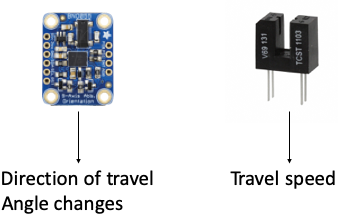
\includegraphics[scale=0.4]{sources/manu_5.png}
\end{columns}
\end{frame}

\begin{frame}{Routing}
\centering
\includegraphics[page=6,scale=0.8]{sources/Rounting_1.pdf}
\end{frame}

\begin{frame}{Routing}
\centering
\includegraphics[page=5,scale=0.55]{sources/Rounting_1.pdf}
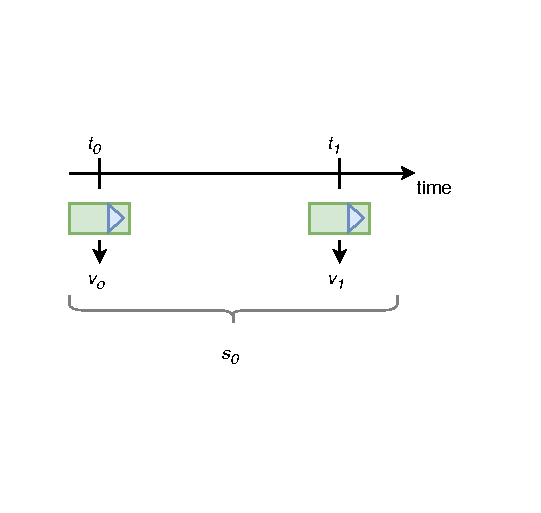
\includegraphics[page=1,scale=0.55]{sources/Rounting_1.pdf}
\end{frame}

\begin{frame}{Routing}
\centering
\includegraphics[page=3,scale=0.8]{sources/Rounting_1.pdf}
\end{frame}

\begin{frame}{Mapping}
\begin{columns}
\column{0.5\textwidth}
\begin{itemize}
\item Ultra sonic sensor
\item Smart movement sensor
\item Related to actual vehicle position and direction of travel
\item Logged coordinates of positions of objects
	\begin{itemize}
	\item Calculated with sensor data
	\end{itemize}
\end{itemize}
\column{0.5\textwidth}
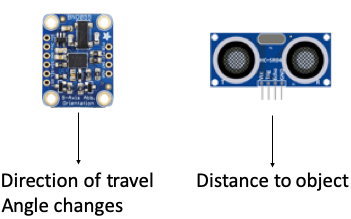
\includegraphics[scale=0.4]{sources/manu_7.png}
\end{columns}
\end{frame}

\begin{frame}{Mapping}
\centering
\includegraphics[page=7,scale=0.8]{sources/Rounting_1.pdf}
\end{frame}

\begin{frame}{Mapping}
\centering
\includegraphics[page=9,scale=0.55]{sources/Rounting_1.pdf}
\includegraphics[page=10,scale=0.55]{sources/Rounting_1.pdf}
\end{frame}

\begin{frame}{Example}
\centering
\frame{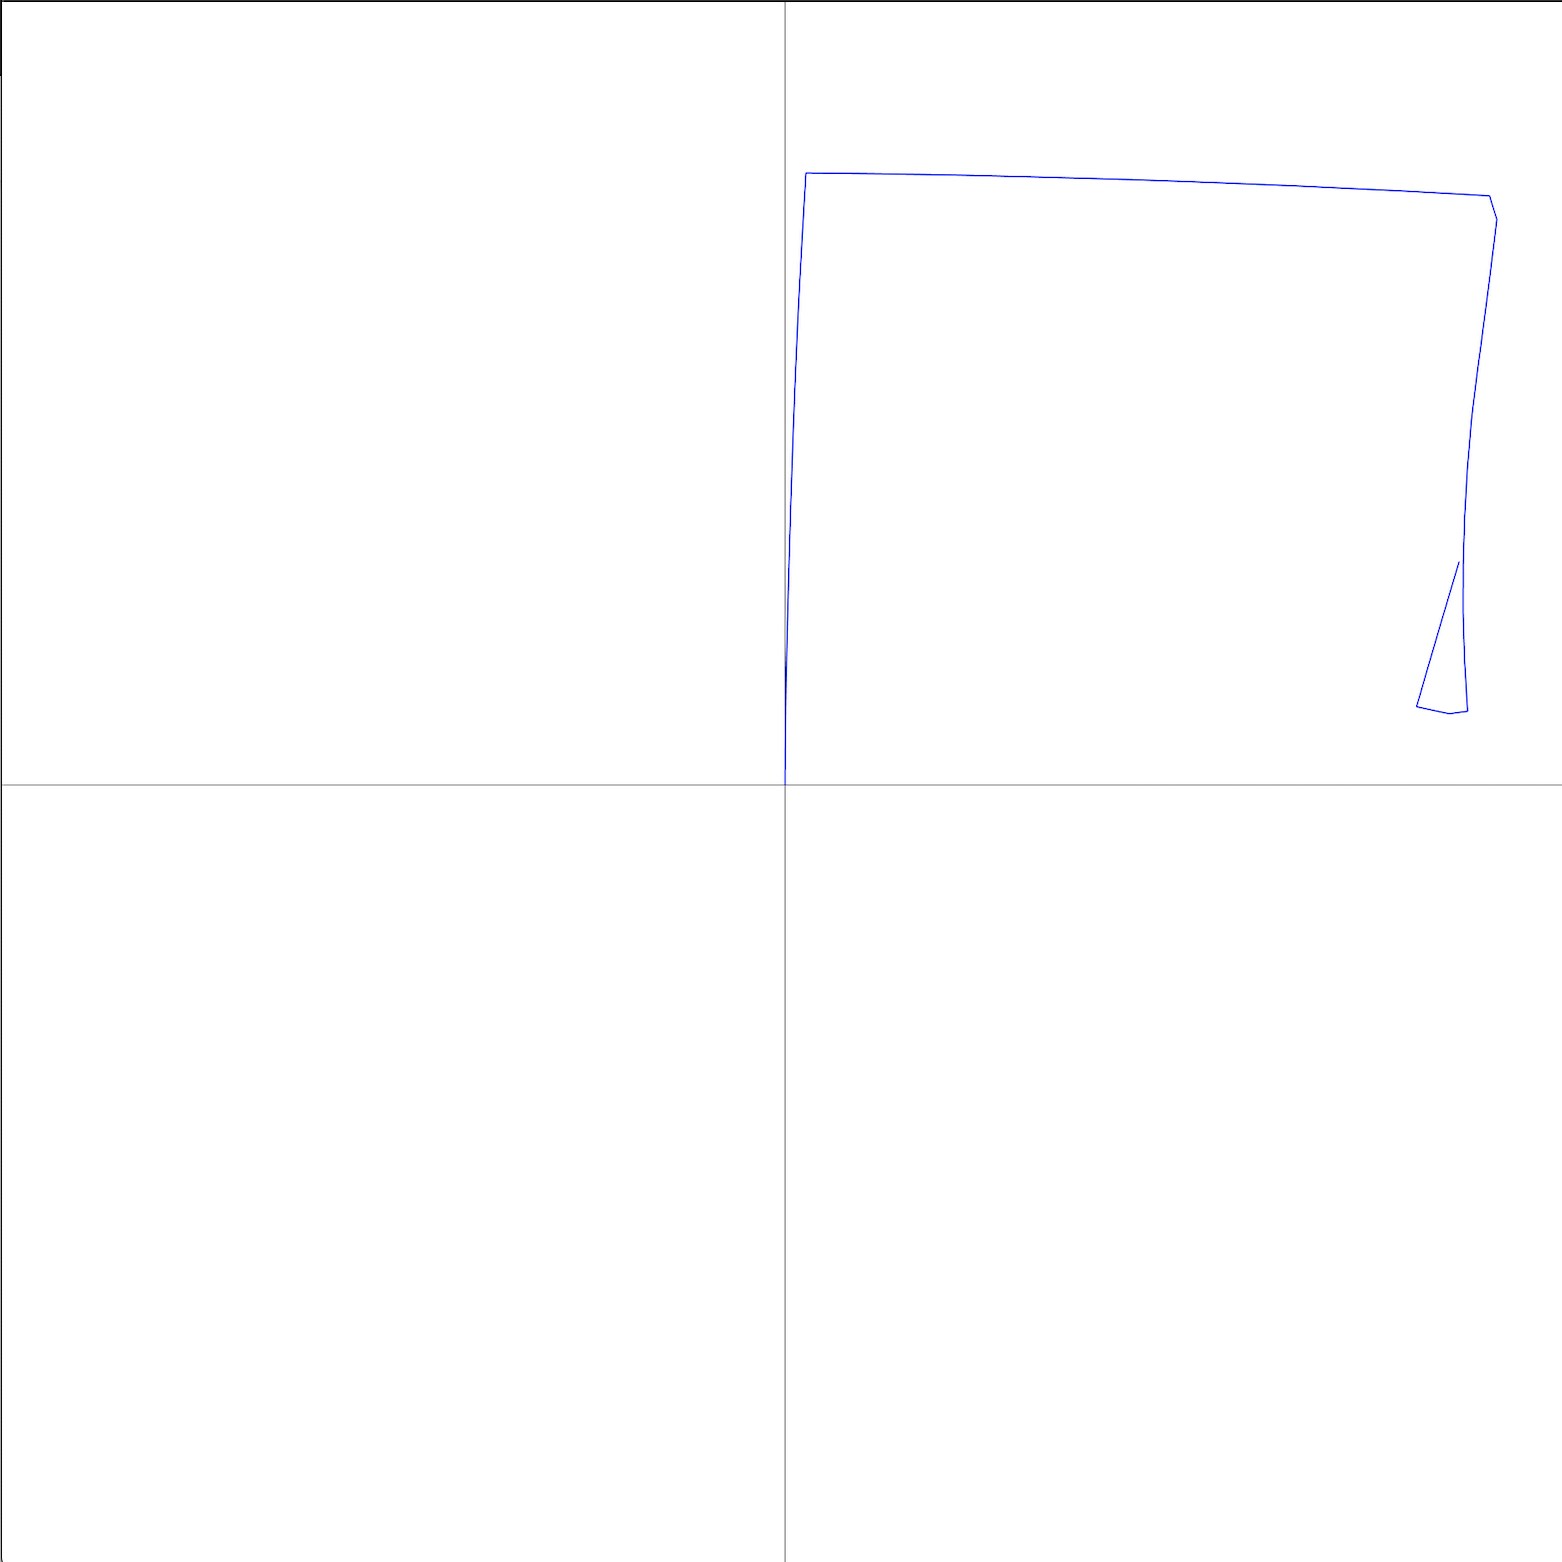
\includegraphics[scale=0.25] {sources/Route_screenshot}}
%\includegraphics[scale=1]{sources/Map.png}
\end{frame}

\begin{frame}{Example}
\centering
\frame{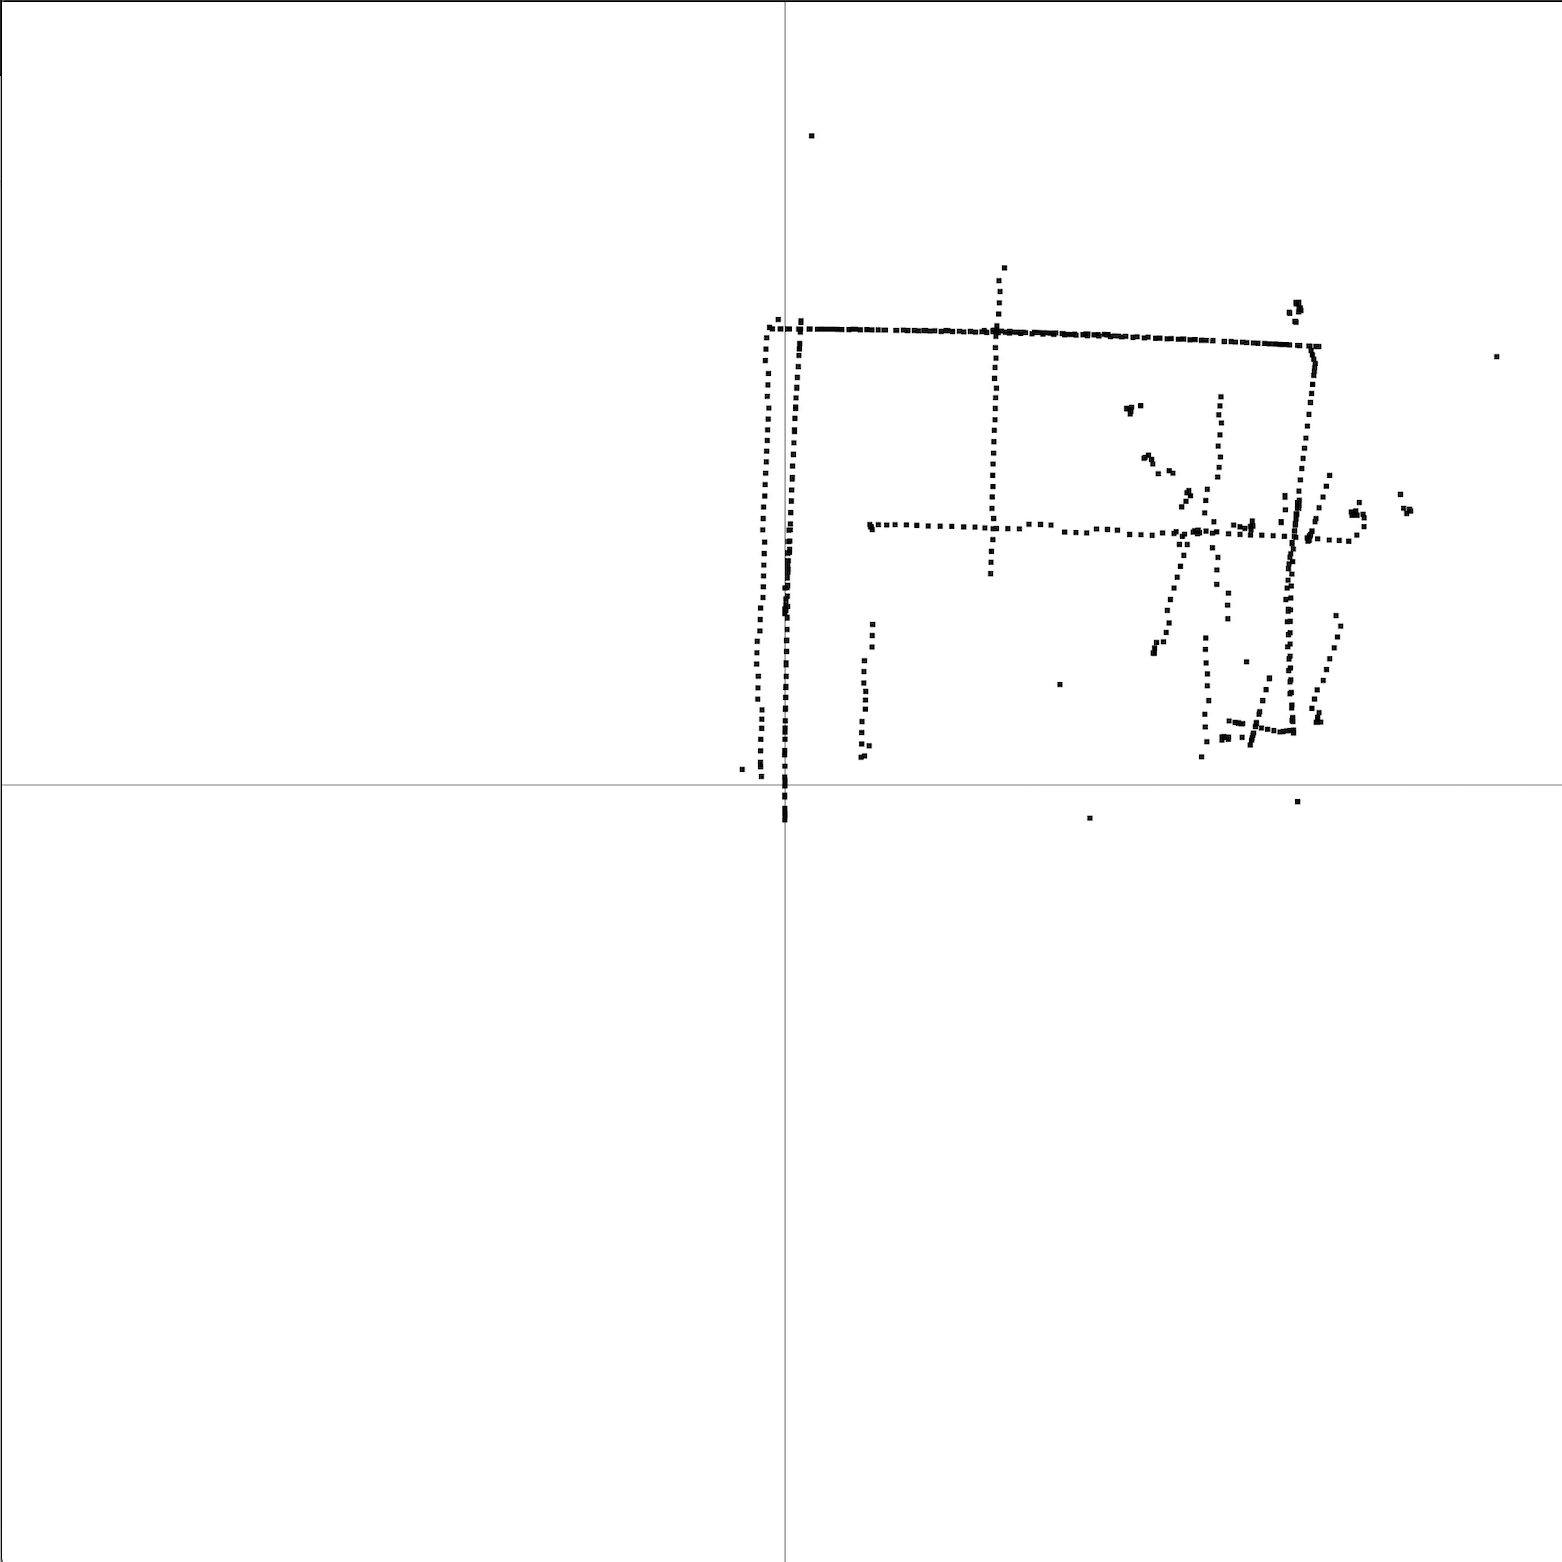
\includegraphics[scale=0.25] {sources/Map_screenshot}}
%\includegraphics[scale=1]{sources/Map.png}
\end{frame}

\section{References}

\begin{frame}{References}
\begin{itemize}
\footnotesize
\item ImageZMQ - \url{https://github.com/jeffbass/imagezmq}
\item Image Processing setup - \url{https://www.pyimagesearch.com/2019/04/15/live-video-streaming-over-network-with-opencv-and-imagezmq/}
\item Tensorflow Modelzoo - \url{https://github.com/tensorflow/models/blob/master/research/object_detection/g3doc/detection_model_zoo.md}
\item SSD - \url{https://arxiv.org/pdf/1512.02325.pdf}
\item MobileNet - \url{https://arxiv.org/pdf/1704.04861.pdf}
\item OpenCV - \url{https://github.com/opencv/opencv/wiki}
\end{itemize}
\vspace{3mm}
For further information please see the \textit{documentation}
\end{frame}

\end{document}

